\begin{figure}[ht!]
\centering
\subfigure{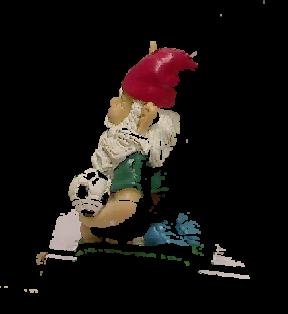
\includegraphics[width=.45\linewidth]{figures/results/100deg}}\quad
\subfigure{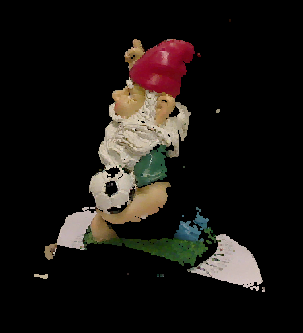
\includegraphics[width=.45\linewidth]{figures/results/80deg}}\\
\subfigure{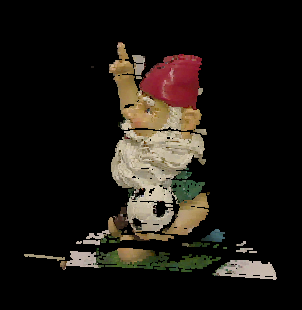
\includegraphics[width=.45\linewidth]{figures/results/60deg}}\quad
\subfigure{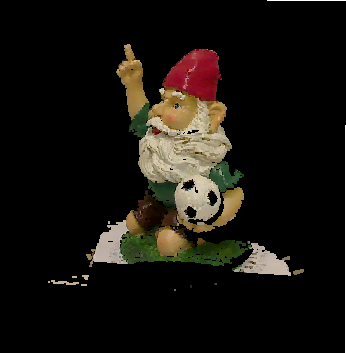
\includegraphics[width=.45\linewidth]{figures/results/40deg}}\\
\subfigure{
\includegraphics[width=.45\linewidth]{figures/results/20deg}}\quad
\subfigure{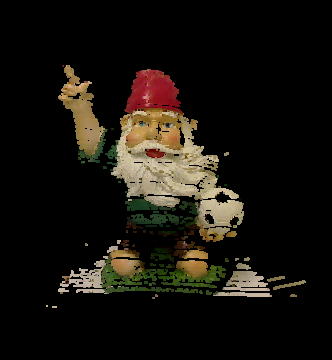
\includegraphics[width=.45\linewidth]{figures/results/0deg}}\\
\caption{Results}
\label{figure:results}
\end{figure}

The imaging system in addition to the source directory, expects a reference
image without the laser stripe and two images of the individual background
patterns used for calibration as input. The program saves the point cloud thus
obtained in a destination directory which is used by the \ac{3DTK} components
for processing and visualization. The results obtained from the
\texttt{show} program are shown in Fig. \ref{figure:results}.

A discernible amount of noise is evident in the final result. However,
considering the quality and the price of the hardware used for the data
acquisition these results can be deemed satisfactory. The gaps in the point
cloud are due to the fast movement of the laser ray over the object. They can
be overcome by reducing the speed of the laser and thereby producing larger
number of image frames. The final step of the software pipeline, namely scan
registration using the ICP method did not yield good results. One possible
explanation is that the rotation angle between the two points from different
scans turned out to be too large making it hard for the \ac{SLAM} component in
\ac{3DTK} to converge.
